\documentclass[10pt]{beamer}

\usepackage{amsmath}
\usepackage{amssymb}
\usepackage{amsthm}
\usepackage[T1]{fontenc}
\usepackage[french]{babel} % traduction
\usepackage[usenames,svgnames,dvipsnames]{xcolor}
\usepackage[hang, small, labelfont=bf, up, textfont=it]{caption} % custom caption under figures
%\usepackage{bookmark}
%\usepackage{booktabs} % beautiful tables
%\usepackage[thicklines]{cancel} % cancel terms in equation
%\usepackage{color} % colors in box (theorems,...)
%\usepackage{enumerate}
\usepackage{float}
\usepackage{framed} % box around text
\usepackage{fancyhdr} % header
%\usepackage{fancyvrb}
\usepackage{mathrsfs}
\usepackage{mathtools}
\usepackage[parfill]{parskip} % avoid bad alignment in paragraphs
\usepackage{pgfplots} % plot in tikz
\usepackage{braket} % braket and sets
\usepackage{derivative} % derivatives
\usepackage{siunitx}
\usepackage{silence} % silence useless warnings
\usepackage{tikz}
\usepackage{tkz-euclide}
\usepackage{tikz-3dplot}
\usepackage{units} % Non-stacked fractions and better unit spacing
\usepackage{xspace} % prints a trailing space in a smart way.

\usetikzlibrary{calc,patterns,angles,quotes}

\tikzset{circ/.style = {fill, circle, inner sep = 0, minimum size = 3}}
\tikzset{scirc/.style = {fill, circle, inner sep = 0, minimum size = 1.5}}
\tikzset{mstate/.style={circle, draw, blue, text=black, minimum width=0.7cm}}

% \titlespacing*{\section}{0pt}{5.5ex plus 1ex minus .2ex}{4.3ex plus .2ex}
% \titlespacing*{\subsection}{0pt}{5.5ex plus 1ex minus .2ex}{4.3ex plus .2ex}

\usepackage{enumitem}
\setlist{nosep,after=\vspace{\baselineskip}}

\pgfplotsset{compat=1.12}
\sisetup{locale = FR}

\usepackage[marginparwidth=2cm]{geometry}
\geometry{
	paper=a4paper,
	inner=2.0cm,
	outer=3.0cm,
	bindingoffset=.5cm,
	top=3.5cm,
	bottom=3.5cm
}

\usepackage{graphicx}
\setkeys{Gin}{width=\linewidth,totalheight=\textheight,keepaspectratio}
%\graphicspath{{figures/}}

% Default images settings
\setkeys{Gin}{width=\linewidth, totalheight=\textheight, keepaspectratio}

%---------------------------------------------------
% BUGGY PACKAGES THAT NEED TO BE LOADED AT THE END
%---------------------------------------------------

% colored hyperlink
% load hyperref at the end to avoid conflicts
\usepackage[colorlinks]{hyperref} % colored ref
% % cleverref must be loaded after hyperref
% \usepackage{cleveref} % create ref

\hypersetup{
  colorlinks=true,
  linkcolor=blue,
  filecolor=blue,
  citecolor=black,
  urlcolor=cyan
}

% conditions for equations
% https://tex.stackexchange.com/questions/95838/how-to-write-a-perfect-equation-parameters-description
\newenvironment{conditions}
  {\par\vspace{\abovedisplayskip}\noindent\begin{tabular}{>{$}l<{$} @{${}={}$} l}}
	{\end{tabular}\par\vspace{\belowdisplayskip}}

\newenvironment{conditions*}
  {\par\vspace{\abovedisplayskip}\noindent
   \tabularx{\columnwidth}{>{$}l<{$} @{${}={}$} >{\raggedright\arraybackslash}X}}
  {\endtabularx\par\vspace{\belowdisplayskip}}

%----------------
% FIX
%----------------

\setlength{\headheight}{14.5pt}

% increase vertical space for aligned equations
\setlength{\jot}{7pt}

% Filter warnings issued by package biblatex starting with "Patching footnotes failed"
\WarningFilter{biblatex}{Patching footnotes failed}

%----------------------
%	COMMANDS
%----------------------

% commands shortcuts
\newcommand{\mb}{\mathbb}
\newcommand{\R}{\mb{R}}
\newcommand{\Z}{\mb{Z}}
\newcommand{\N}{\mb{N}}
\newcommand{\C}{\mb{C}}
\newcommand{\A}{\mb{A}} % hypersphere area
\newcommand{\V}{\mb{V}} % hypersphere volume
\newcommand{\dS}{\cdot d\vb{S}}
\newcommand{\lag}{\mathcal{L}}
\newcommand{\ham}{\mathcal{H}}
\newcommand{\Mod}[1]{\ \mathrm{mod}\ #1}

\renewcommand{\vec}[1]{\mathbf{#1}} % bold vectors
\newcommand{\vd}[1]{\dot{\vec{#1}}}
\newcommand{\vdd}[1]{\ddot{\vec{#1}}}

% norm
\newcommand{\bignorm}[1]{\left\lVert#1\right\rVert}

% smaller overline (line above variable)
\newcommand{\overbar}[1]{\mkern 1.5mu\overline{\mkern-1.5mu#1\mkern-1.5mu}\mkern 1.5mu}

% prints an asterisk that takes up no horizontal space.
% useful in tabular environments.
\newcommand{\hangstar}{\makebox[0pt][l]{*}}

% Prints argument within hanging parentheses (i.e., parentheses that take
% up no horizontal space). Useful in tabular environments.
\newcommand{\hangp}[1]{\makebox[0pt][r]{(}#1\makebox[0pt][l]{)}}

% cancel terms with color
% \newcommand{\ccancel}[2]{\renewcommand{\CancelColor}{\color{#2}}\bcancel{#1}}

% small parallel
\makeatletter
\newcommand{\newparallel}{\mathrel{\mathpalette\new@parallel\relax}}
\newcommand{\new@parallel}[2]{%
  \begingroup
  \sbox\z@{$#1T$}% get the height of an uppercase letter
  \resizebox{!}{\ht\z@}{\raisebox{\depth}{$\m@th#1/\mkern-5mu/$}}%
  \endgroup
}
\makeatother

\renewcommand*\contentsname{Table des matières}

\usetheme{Copenhagen}
\usecolortheme{default}

\title{Mécanique Céleste}
\subtitle{Évolution orbitale du Soleil, de Jupiter et de Saturne}
\author{M. Rousseau \and M. Volders}

\institute{
  Faculté des Sciences\\
  Université Catholique de Louvain
}

\date{09-06-2021}

% Use a simple TikZ graphic to show where the logo is positioned
\logo{
\includegraphics[scale=0.15]{figures/institution.png}}

\AtBeginSection[]
{
  \begin{frame}
    \frametitle{Table of Contents}
    \tableofcontents[currentsection]
  \end{frame}
}

\begin{document}
\frame{\titlepage}

\begin{frame}{Sommaire}
\begin{enumerate}
    \item Énoncé du problème
    \item Méthodes numériques utilisées
    \item Évolution orbitale
    \item Quantités conservées
\end{enumerate}
\end{frame}

\begin{frame}{Problème à $2$ corps}
% \begin{center}
%   \begin{tikzpicture}[scale=1]
%     % help lines
%     \draw [help lines] (0,0) grid (2,2);
%     % origin
%     \node[below] at (0,0) {$O$};
%     % r_1
%     \draw[->,thick] (0,0) -- (0.1,1.2);
%     \filldraw[black] (0.1,1.2) circle 2pt node[anchor=left] {$m_1$};
%     \node[left] at (0,0.6)  {$\vec{r}_1$};
%     % r_2
%     \draw[->,thick] (0,0) -- (1.5,0.8);
%     \filldraw[black] (1.5,0.8) circle 2pt node[anchor=right] {$m_2$};
%     node[right] at (1.6,0.4)  {$\vec{r}_2$};
%     % r_1 - r_2
%     \draw (1.5,0.8) -- (0.1,1.2)
%     \node[below] {0.7,1.3} {$|\vec{r}_1 - \vec{r}_2|$};
% \end{tikzpicture}
% \end{center}

\begin{block}{Hamiltonien à $2$ corps}
  \begin{equation}
    \ham = \frac{\vec{p}_1^2}{2m_1} + \frac{\vec{p}_2^2}{2m_2} - \frac{Gm_1m_2}{|\vec{r}_1 - \vec{r}_2|}
  \end{equation}
\end{block}

A partir des équations canoniques pour un Hamiltonien quelconque, on peut trouver un système d'équations différentielles.
\begin{equation}
  \dot{p}_i = -\pdv{\ham}{r_i} \quad ; \quad \dot{r_i} = \pdv{\ham}{p_i}
\end{equation}
pour $i = \set{x,y,z}$ et $(r_x, r_y, r_z) = (x, y, z)$.

\end{frame}

\begin{frame}{Généralisation à $N$ corps}
\begin{itemize}
  \item Ajouter des corps célestes à notre simulation sans avoir à redériver les équations différentielles.
  \item On doit tenir compte des potentiels d'interactions entre les différentes masses.
\end{itemize}

\begin{block}{Hamiltonien à N corps}
  \begin{equation}
    \ham = \sum_{i=1}^N \frac{\vec{p}_i^2}{2m_i} + \sum_{1\leq i<j \leq N} \frac{Gm_i m_j}{|\vec{r}_i - \vec{r}_j|}
  \end{equation}
  où $|\vec{r}_i - \vec{r}_j|$ est la distance relative entre la masse $m_i$ et la masse $m_j$.
\end{block}

\end{frame}

\begin{frame}{Équations canoniques}
Système d'équations différentielles :
\begin{align}
  \vd{r}_i =
  \begin{pmatrix}
    \dot{x}_i \\ \dot{y}_i \\ \dot{z}_i
  \end{pmatrix}
  =
  \begin{pmatrix}
    \frac{p_{x_i}}{m_i} \\[6pt]
    \frac{p_{y_i}}{m_i} \\[6pt]
    \frac{p_{z_i}}{m_i}
  \end{pmatrix}
\end{align}
\begin{align}
  \vd{p}_i =
  \begin{pmatrix}
    \dot{p}_{x_i} \\ \dot{p}_{y_i} \\ \dot{p}_{z_i}
  \end{pmatrix}
  =
  \begin{pmatrix}
    \sum_{j \neq i}^{N} - \frac{Gm_im_j}{(\vec{r}_{ij})^3} (x_i - x_j) \\[6pt]
    \sum_{j \neq i}^{N} - \frac{Gm_im_j}{(\vec{r}_{ij})^3} (y_i - y_j) \\[6pt]
    \sum_{j \neq i}^{N} - \frac{Gm_im_j}{(\vec{r}_{ij})^3} (z_i - z_j)
  \end{pmatrix}
\end{align}
\end{frame}

\begin{frame}
\frametitle{Schémas numériques}
Schéma "classique" (famille des Runge-Kutta) :
\begin{itemize}
  \item Heun (\textit{ordre $2$})
\end{itemize}
Schémas symplectiques :
\begin{itemize}
  \item Euler symplectique (\textit{ordre $1$})
  \item Stormer-Verlet (\textit{ordre $2$})
\end{itemize}
\end{frame}

\begin{frame}{Évolution orbitale}
  \begin{figure}
      \centering
      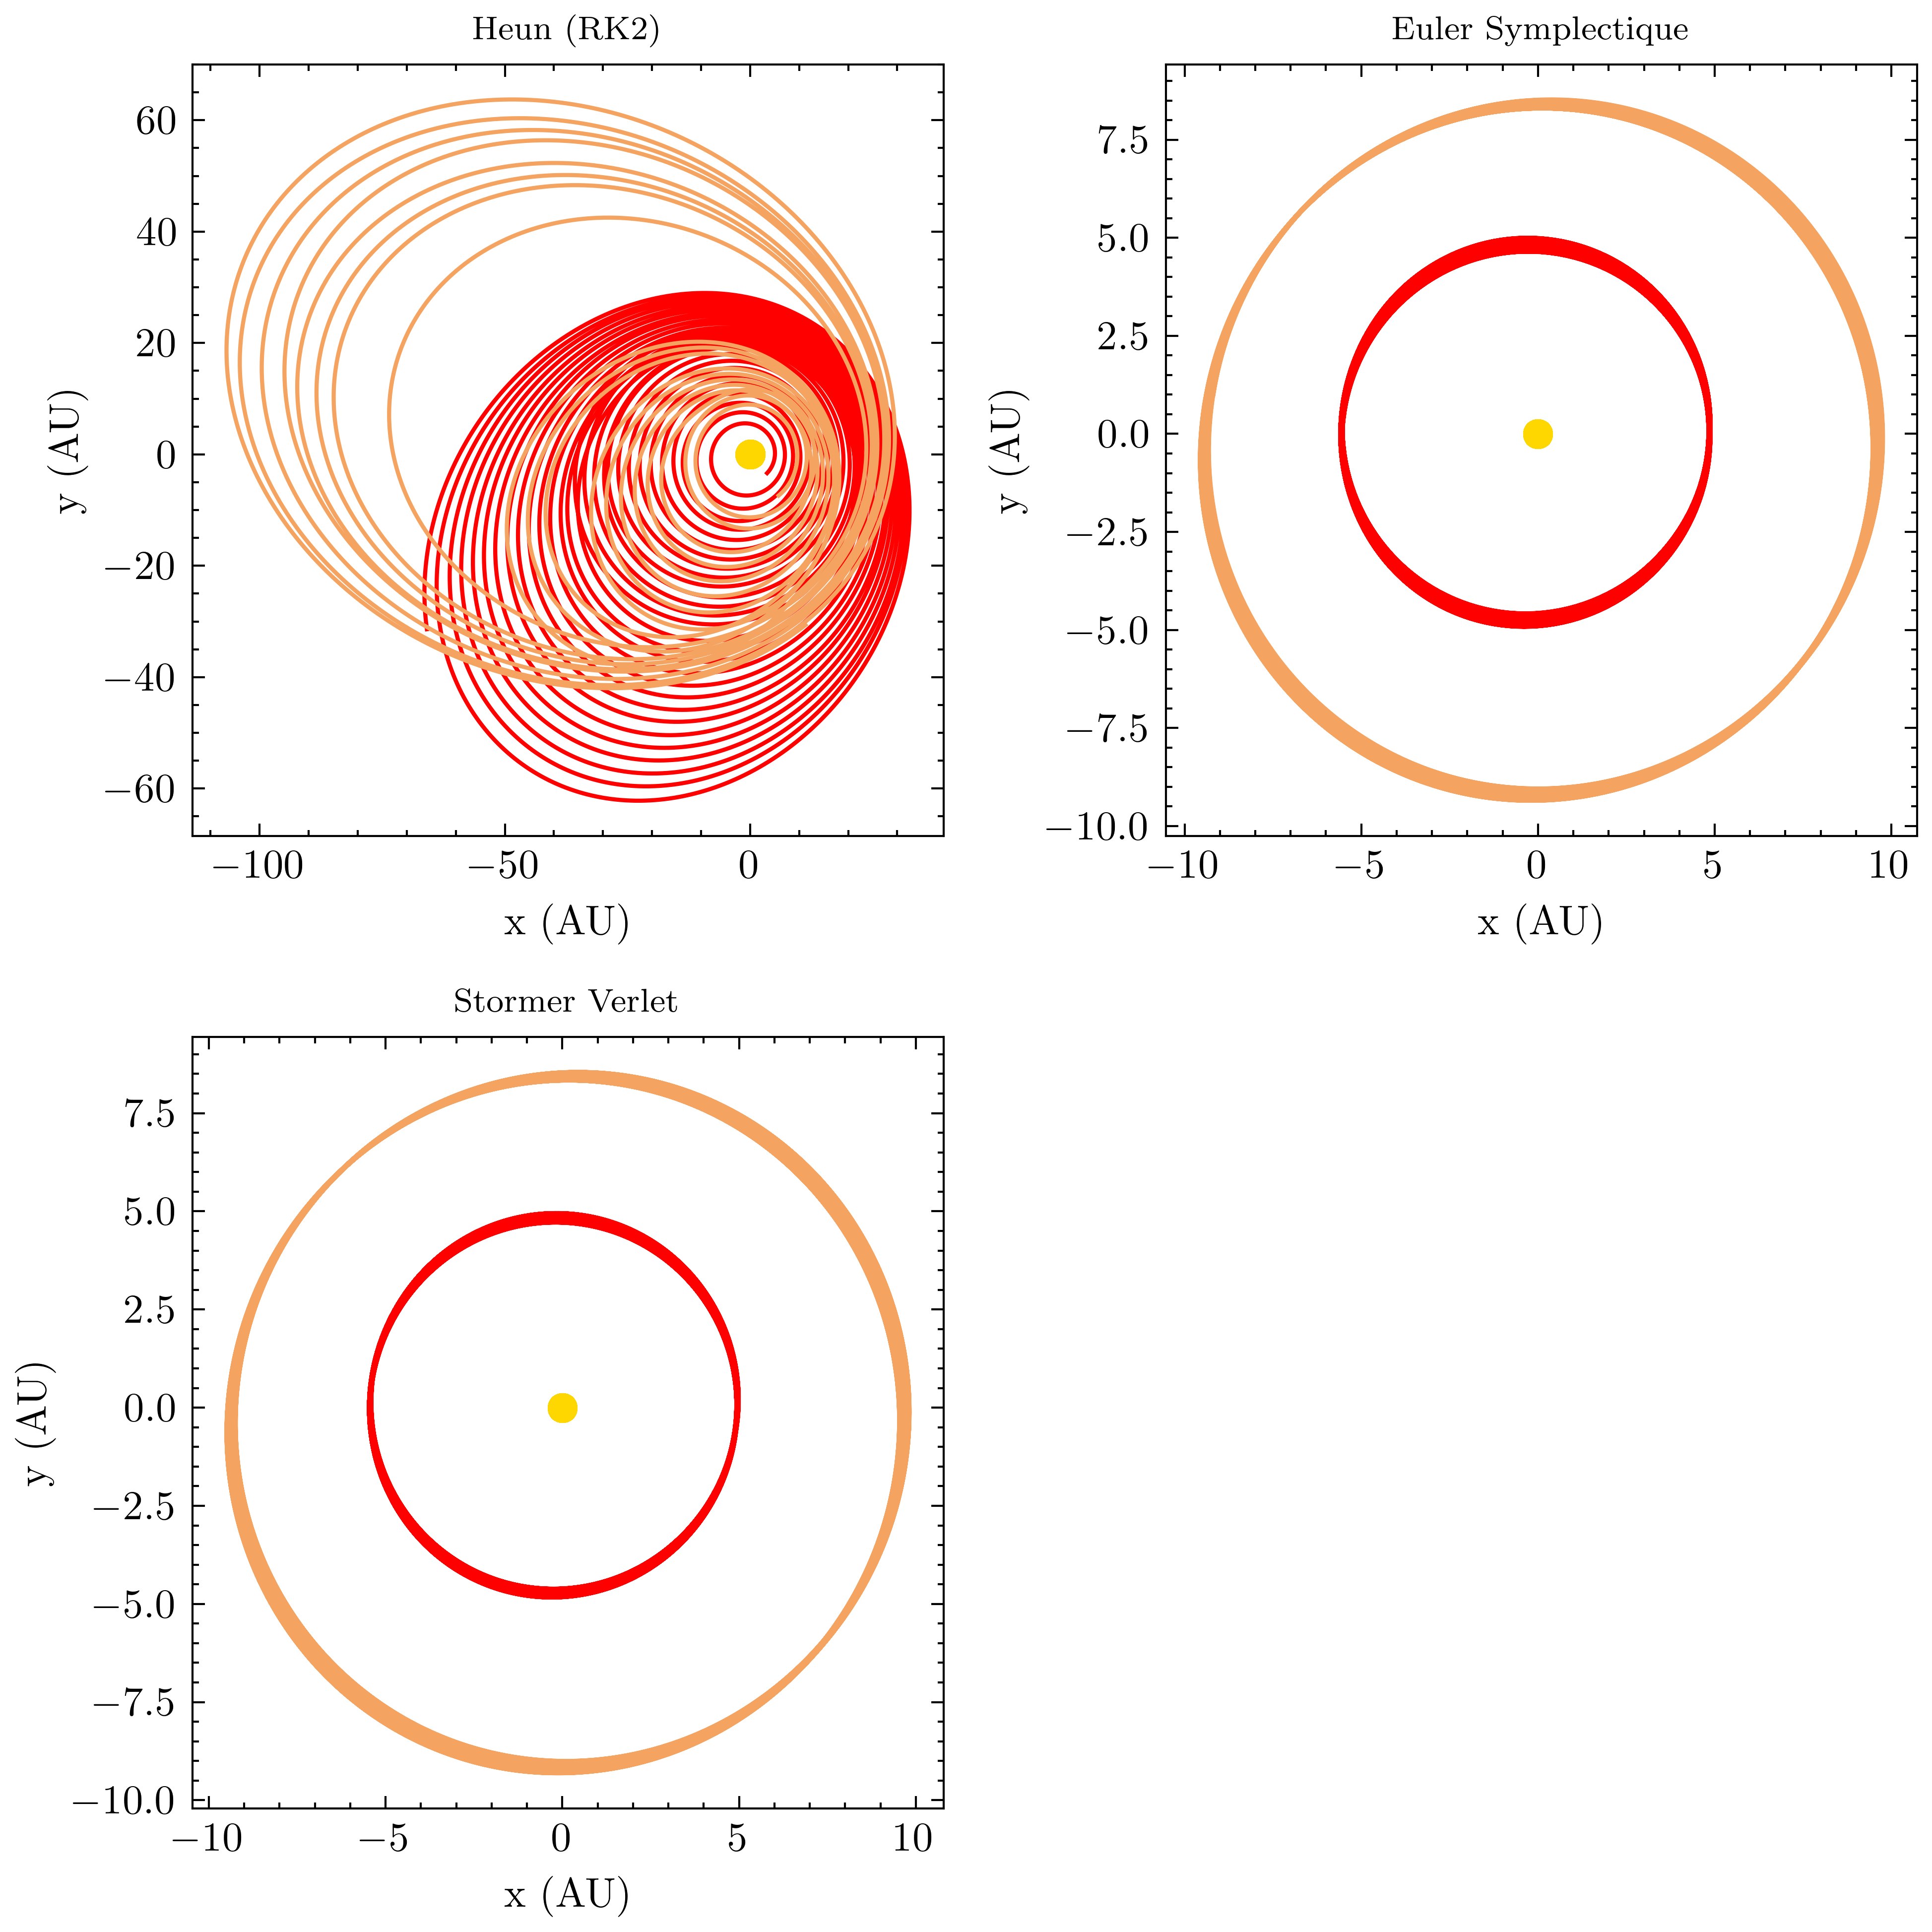
\includegraphics[width=\textwidth,height=0.7\textheight,keepaspectratio]{figures/5000_years/orbital-plot2d.png}
      \caption{Evolution orbitale en 2 dimension de l'orbite du Soleil (\emph{point jaune}), de Jupiter (\emph{rouge}) et de Saturne (\emph{brun}) pour les $5000$ prochaines années.}
      \label{fig:plot2D--5000}
  \end{figure}
\end{frame}

\begin{frame}{Evolution orbitale}
  \begin{figure}
    \centering
    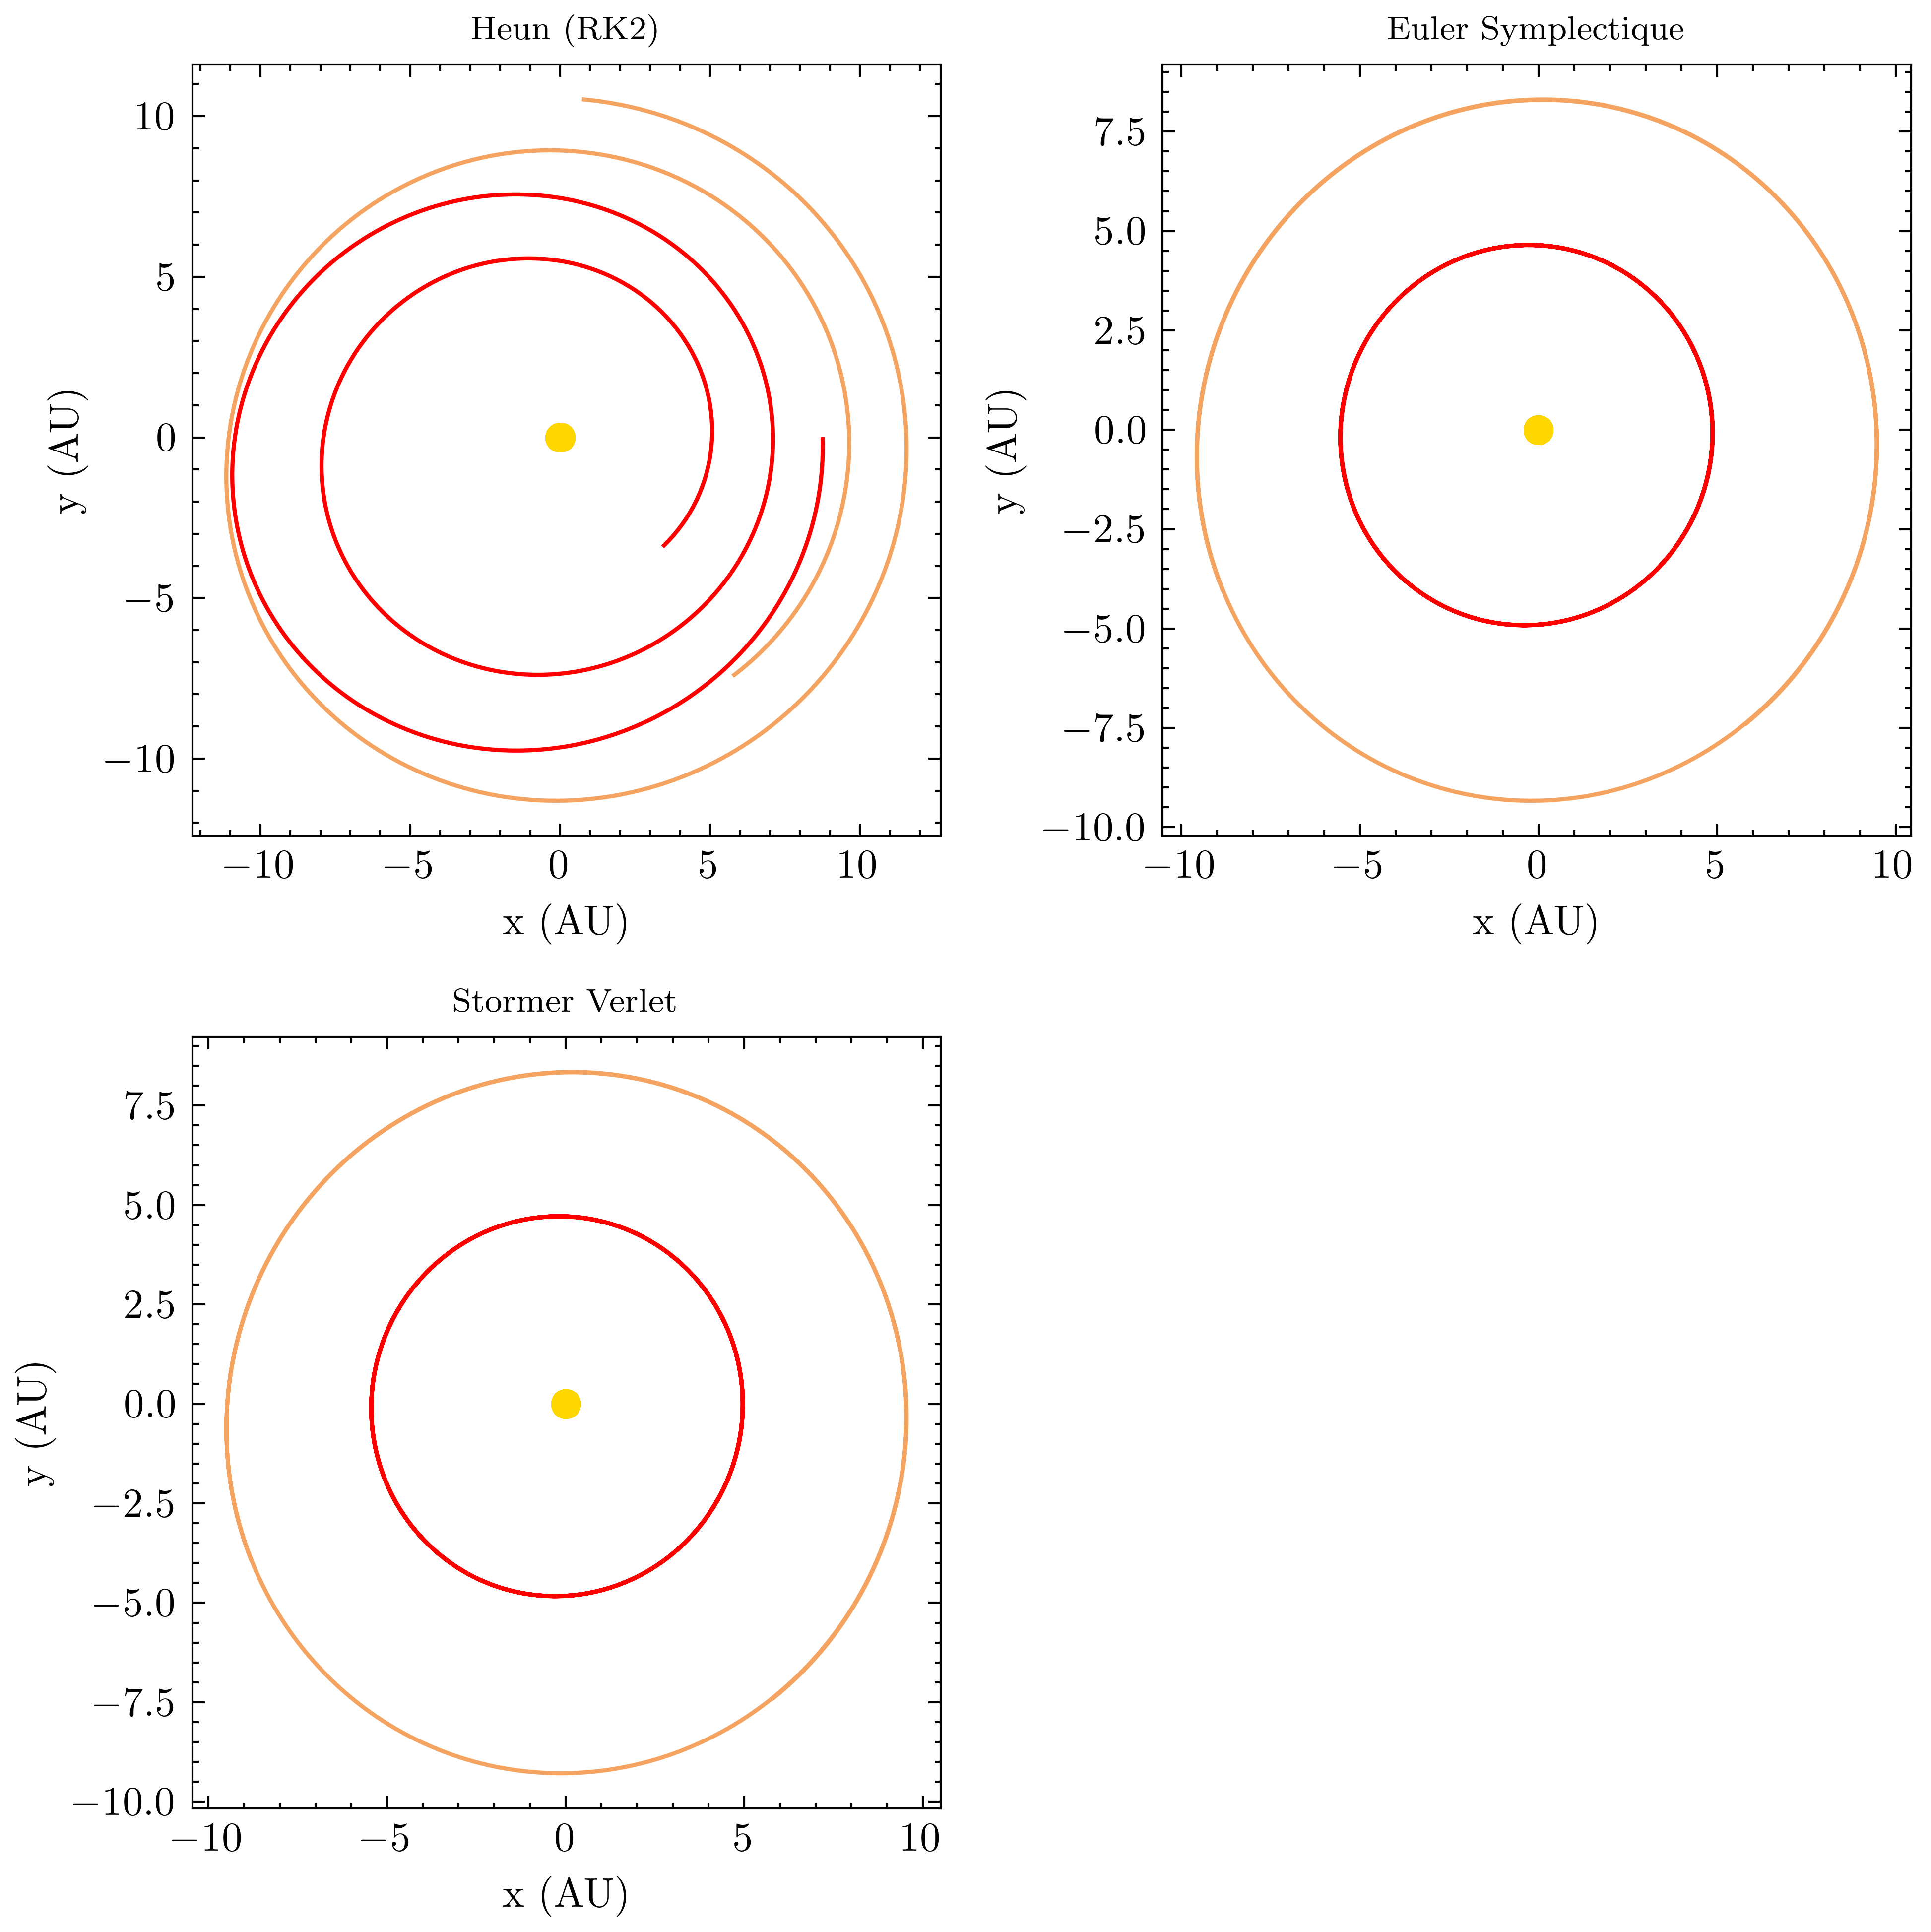
\includegraphics[width=\textwidth,height=0.7\textheight,keepaspectratio]{figures/50_years/orbital-plot2d.png}
    \caption{Evolution orbitale en 2 dimension de l'orbite du Soleil (\emph{point jaune}), de Jupiter (\emph{rouge}) et de Saturne (\emph{brun}) pour les $50$ prochaines années.}
    \label{fig:plot2D--50}
  \end{figure}
\end{frame}

\begin{frame}{Conservation de l'énergie}
  \begin{figure}
    \centering
    \includegraphics[width=\textwidth,height=0.7\textheight,keepaspectratio]{figures/5000_years/orbital-energy.pdf}
    \caption{Variation de l'énergie du système du système à 3 corps sur \textbf{$5000$ années} pour les différents schémas numériques utilisés.}
    \label{fig:orbital-energy--5000}
  \end{figure}
\end{frame}

\begin{frame}{Conservation de l'énergie}
  \begin{figure}
    \centering
    \includegraphics[width=\textwidth,height=0.7\textheight,keepaspectratio]{figures/50_years/orbital-energy.pdf}
    \caption{Variation de l'énergie du système à 3 corps sur \textbf{$50$ années} pour les différents schémas numériques utilisés.}
    \label{fig:orbital-energy--50}
  \end{figure}
\end{frame}

\begin{frame}{Conservation du moment angulaire}
  \begin{equation}
    \vec{L} = \sum_{i=1}^N \vec{l}_i = \sum_{i=1}^N \vec{r}_i \times m_i \vec{v}_i
  \end{equation}
  \begin{figure}
    \centering
    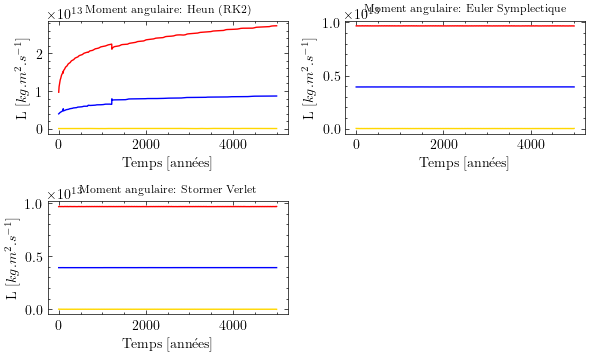
\includegraphics[width=\textwidth,height=0.5\textheight,keepaspectratio]{figures/5000_years/orbital-angular-momentum.pdf}
    \caption{Conservation du moment angulaire en fonction du temps du système à 3 corps pour les différents schémas numériques utilisés.}
    \label{fig:orbital-angular-momentum}
  \end{figure}
\end{frame}

\begin{frame}{Conservation du moment angulaire}
  S'il y conservation du moment angulaire, le mouvement orbital est plan.
  \begin{figure}
    \centering
    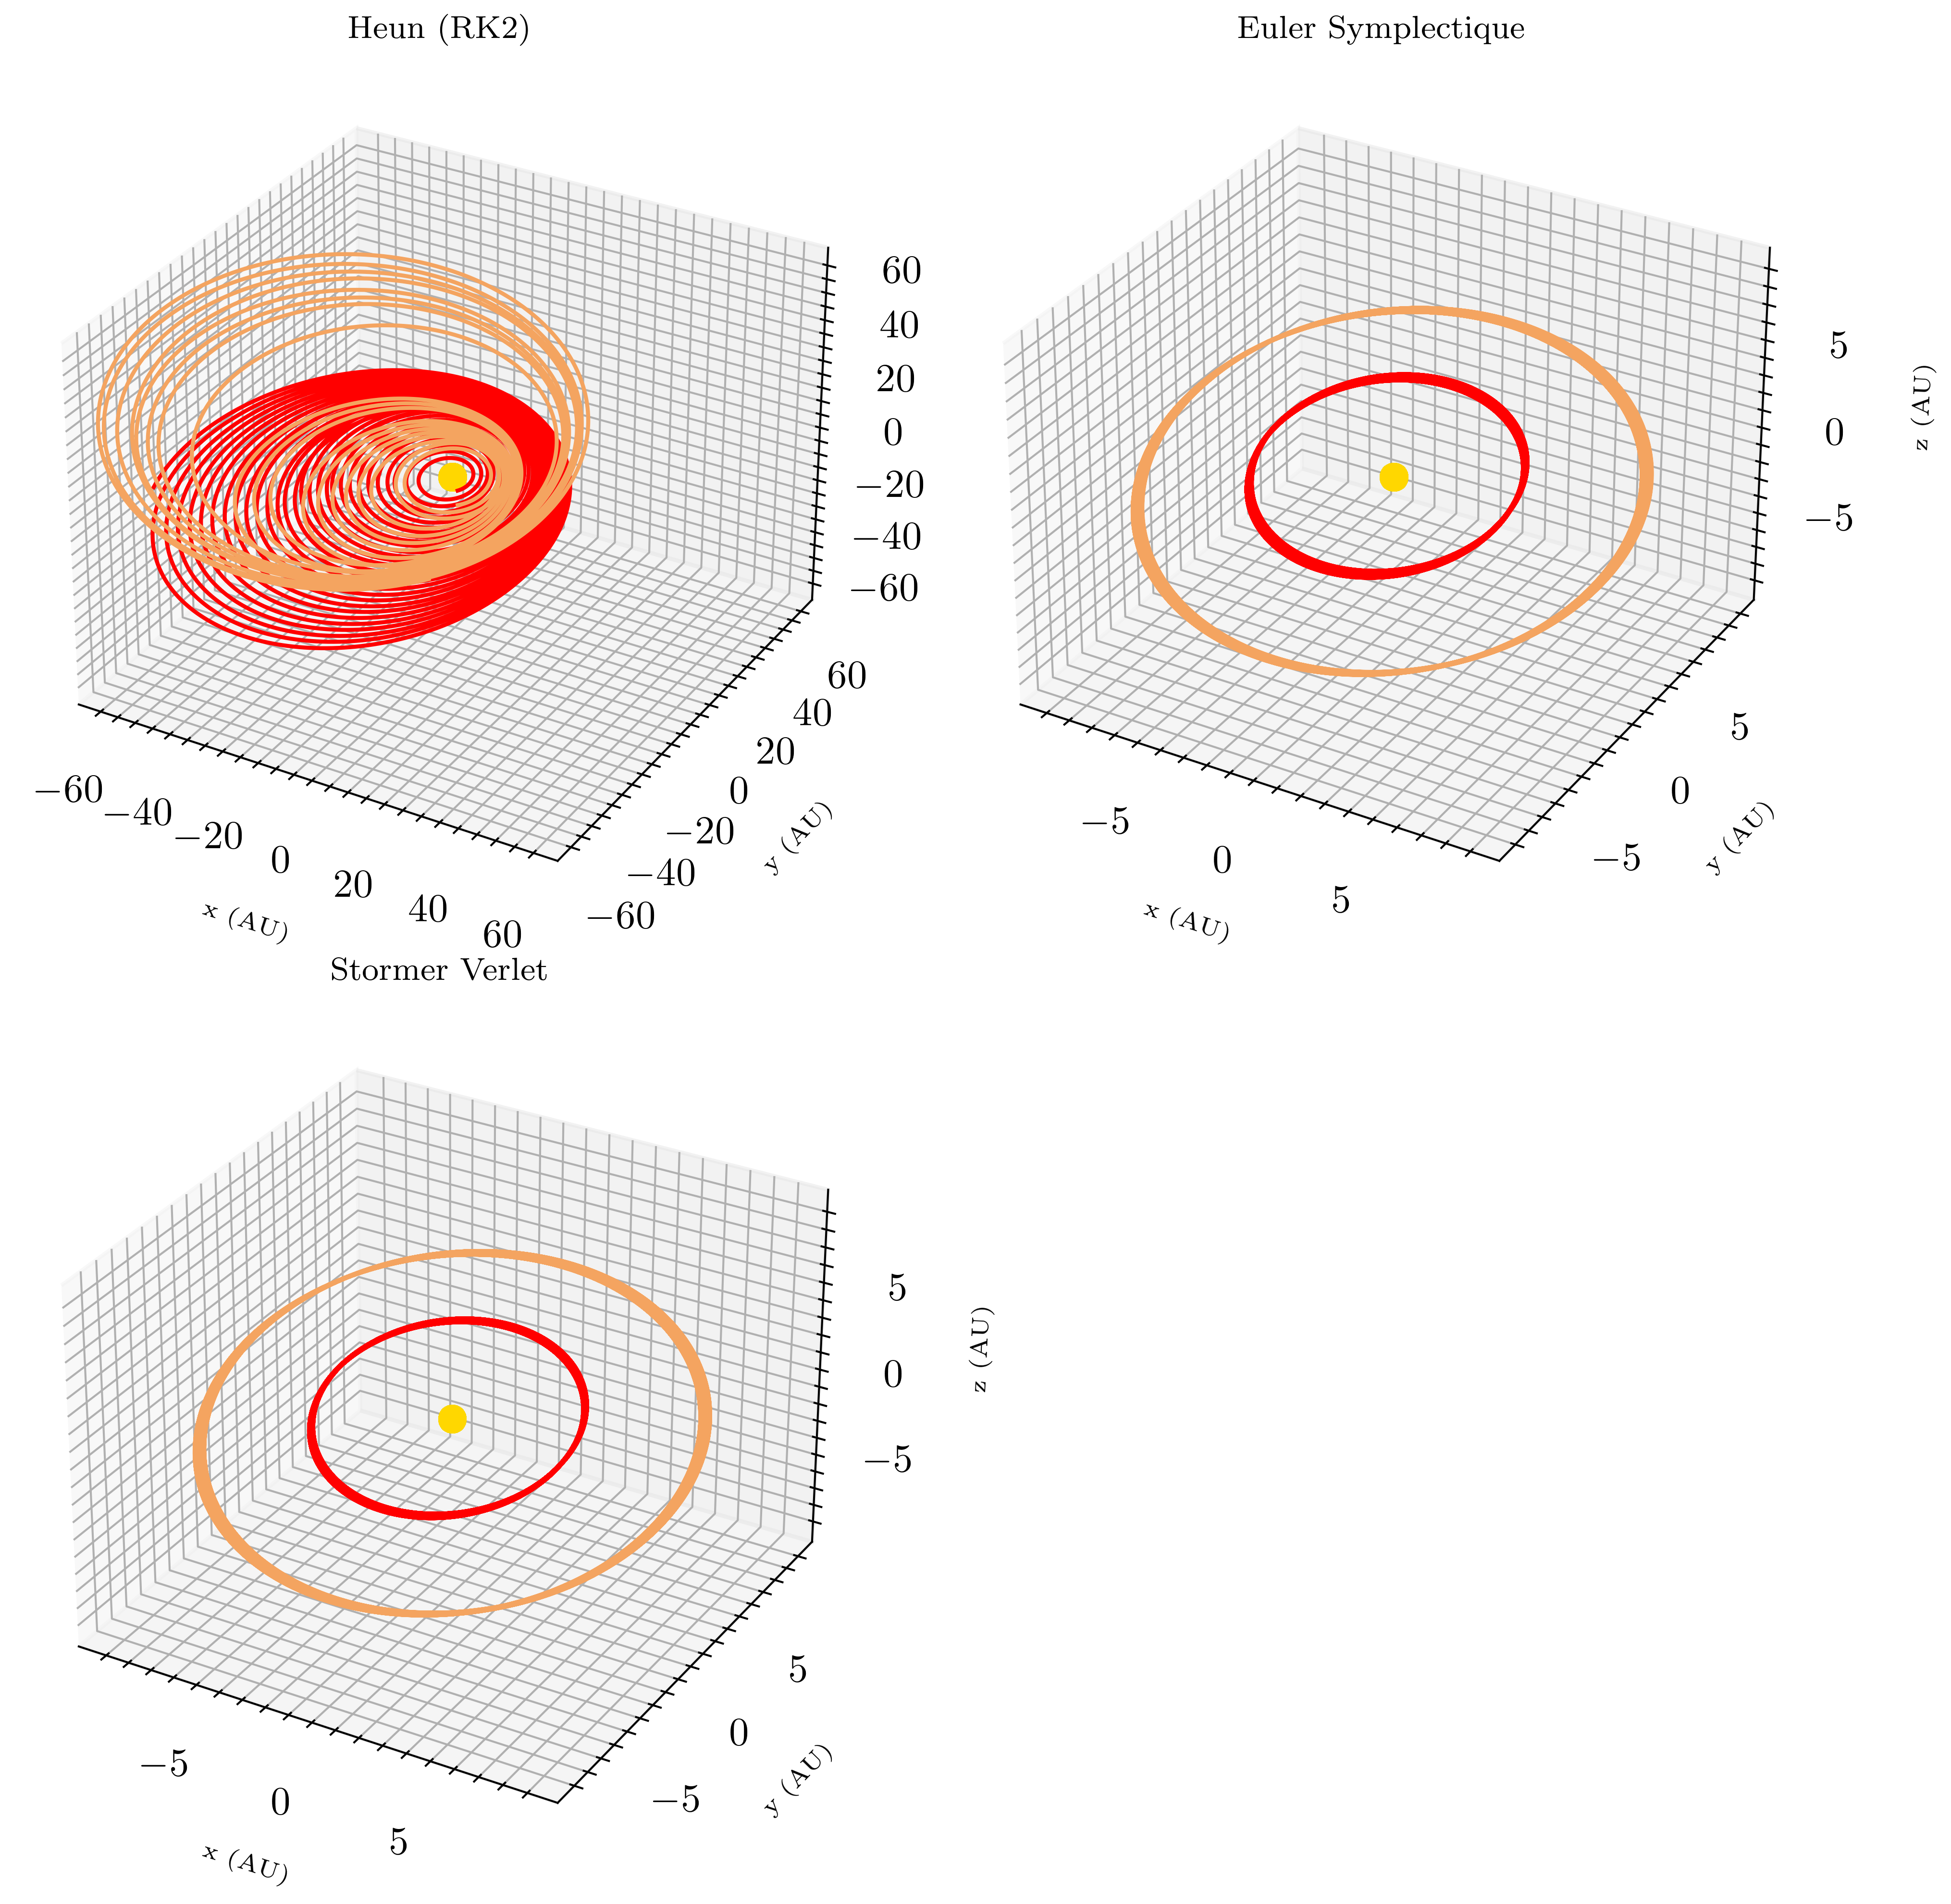
\includegraphics[width=\textwidth,height=0.5\textheight,keepaspectratio]{figures/5000_years/orbital-plot3d.png}
    \caption{Evolution orbitale en $3$ dimension de l'orbite du Soleil (\emph{point jaune}), de Jupiter (\emph{rouge}) et de Saturne (\emph{brun}) pour les $5000$ prochaines années.}
    \label{fig:orbital-plot3D--5000}
  \end{figure}
\end{frame}

\begin{frame}{Surface totale balayée}

\begin{center}
    \begin{tikzpicture}[scale=2]
    \draw(0,0)--node[below]{$\vec{r}_1$} (1.7,0)
        --node[above]{$\vec{r}_2$}(0,1)
        --node[left]{$r_2 d\theta$}(0,0);
    \draw[very thin,<->](1.4,0) arc [start angle=180,end angle=150, radius=0.3];
    \node at (1.3,0.1){$d\theta$};
  \end{tikzpicture}
\end{center}

\begin{align}
  dA &\approx \frac{1}{2} ||\vec{r}_1|| ||\vec{r}_2|| d\theta, \quad d\theta \ll 1
\end{align}

Aire balayée entre $2$ temps successifs $t_j$ et $t_{j+1}$, $j \in \Z$ :
\begin{equation}
  \Delta A \approx \frac{1}{2} ||\vec{r}_1|| ||\vec{r}_2|| \Delta \theta
\end{equation}

\end{frame}

\begin{frame}
  \begin{figure}
    \centering
    \includegraphics[width=\textwidth,height=0.7\textheight,keepaspectratio]{figures/5000_years/orbital-total_area_swept.pdf}
    \caption{Somme des surfaces balayées par les différentes planètes pour les \textbf{$5000$ prochaines années} et ce pour les différents schémas numériques utilisés.}
    \label{fig:orbital-total_area_swept--5000}
  \end{figure}
\end{frame}

\begin{frame}{Surface totale balayée}
  \begin{figure}
    \centering
    \includegraphics[width=\textwidth,height=0.7\textheight,keepaspectratio]{figures/50_years/orbital-total_area_swept.pdf}
    \caption{Somme des surfaces balayées par les différentes planètes pour les \textbf{$50$ prochaines années} et ce pour les différents schémas numériques utilisés.}
    \label{fig:orbital-total_area_swept--50}
  \end{figure}
\end{frame}

\begin{frame}{Conclusion}
  Schémas non-symplectiques :
  \begin{itemize}
    \item Peuvent monter à des ordres très élevés (en particulier les \textbf{Runge-Kutta}).
    \item Ne conservent pas l'énergie sur des longs temps d'intégration.
    \item Orbites des planètes dévient de leur trajectoire.
  \end{itemize}

  Schéma symplectiques :
  \begin{itemize}
    \item Plus difficile d'implémenter des schémas d'ordre élevés.
    \item Ne conservent pas \textbf{exactement l'énergie} mais conservent l'énergie en moyenne.
    \item Orbites des planètes sont stables et ne subissent que de légères fluctuations.
  \end{itemize}
\end{frame}

\end{document}
